% Created 2019-03-05 Tue 02:16
\documentclass[11pt]{article}
\usepackage[utf8]{inputenc}
\usepackage[T1]{fontenc}
\usepackage{fixltx2e}
\usepackage{graphicx}
\usepackage{longtable}
\usepackage{float}
\usepackage{wrapfig}
\usepackage{rotating}
\usepackage[normalem]{ulem}
\usepackage{amsmath}
\usepackage{textcomp}
\usepackage{marvosym}
\usepackage{wasysym}
\usepackage{amssymb}
\usepackage{hyperref}
\tolerance=1000
\usepackage{minted}
\usepackage{amsthm}
\usepackage[margin=1.0in]{geometry}
\setlength{\parindent}{0pt}
\setlength{\parskip}{\baselineskip}
\author{Thomas Alford}
\date{\today}
\title{Ph21 Problem Set 4}
\hypersetup{
  pdfkeywords={},
  pdfsubject={},
  pdfcreator={Emacs 25.2.1 (Org mode 8.2.10)}}
\begin{document}

\maketitle
\section*{Problem 1}
\label{sec-1}
\subsection*{Imports}
\label{sec-1-1}
\begin{minted}[frame=lines,fontsize=\scriptsize]{python}
import numpy as np
import matplotlib.pyplot as plt
%matplotlib inline
import dynesty
from dynesty import plotting as dyplot
\end{minted}

\subsection*{Previous Code}
\label{sec-1-2}

\begin{minted}[frame=lines,fontsize=\scriptsize]{python}
def biased_flip(H, size=None):
    return np.random.random(size=size) < H

def get_H_vals(H):
    nval = 1024
    bflips = biased_flip(H, size=nval)
    sum_val = np.sum(bflips)
    return sum_val, nval

def get_H_prob(n, h, H):
    if (H <= 0 or H >= 1):
        return 0
    return (np.math.factorial(n) / (np.math.factorial(h) * np.math.factorial(
        n - h))) * H ** h * (1 - H) ** (n - h)
\end{minted}

\subsection*{MCMC Runs}
\label{sec-1-3}

At this point in using Dynesty the main parameters to vary are nlive and
dlogz. nlive increases the number of live points, which gives a more accurate
posterior but requires more iterations to converge. dlogz is the change in
log-likelihood between samples at which we stop. So, smaller values result in
more iterations.

\begin{minted}[frame=lines,fontsize=\scriptsize]{python}
def plot_H_probs(real_H, sampler_results, prior_func, dlogz, nlive, 
                 **prior_kwargs):
    fig, (ax1, ax2) = plt.subplots(2, 1, figsize=(8, 7))
    ax1.plot(sampler_results.samples, np.exp(sampler_results.logl), '.',
            label='n=1024')
    H_vals = np.linspace(0, 1, 1000)
    prior_vals = np.array([prior_func(H, **prior_kwargs) for H in H_vals])
    normed_vals = prior_vals * (np.max(np.exp(
        sampler_results.logl)) / np.max(prior_vals))
    ax1.plot(H_vals, normed_vals, '--', label='prior')
    ax1.set_ylabel('likelihood')
    ax1.legend()

    ax2.hist(sampler_results.samples, density=True, bins=1000)
    #ax2.set_xlabel('H')
    ax2.set_ylabel('sample density')

    plt.suptitle('Posterior probabilities of H with real H=%s, '
                 'dlogz=%s, nlive=%s' % (real_H, dlogz, nlive))
    fig.text(0.5, 0.04, 'Number of Heads', ha='center')
    #fig.text(0.04, 0.5, 'Posterior Density', va='center', rotation='vertical')
    plt.subplots_adjust(top=0.9, hspace=.6)
    plt.show()

def get_and_plot_H(H, prior_func, dlogz_val, nlive_val, **prior_kwargs):
    sum_val, nval = get_H_vals(H)

    def loglike(H):
        return np.log(get_H_prob(nval, sum_val, H[0]))

    def ptform(u):
        return u

    ndim = 1
    sampler = dynesty.NestedSampler(loglike, ptform, ndim,
                                           bound='single', nlive=nlive_val) 

    sampler.run_nested(dlogz=dlogz_val, print_progress=False)
    results = sampler.results
    plot_H_probs(H, results, prior_func, dlogz_val, nlive_val, **prior_kwargs)
    return results.samples[-1, 0]
    
def uniform_prior(H):
    return 1
\end{minted}

\subsubsection*{Uniform Priors}
\label{sec-1-3-1}

\begin{itemize}
\item Testing Nlive
\label{sec-1-3-1-1}

\begin{minted}[frame=lines,fontsize=\scriptsize]{python}
maxL = get_and_plot_H(.5, uniform_prior, 1, 10)
\end{minted}

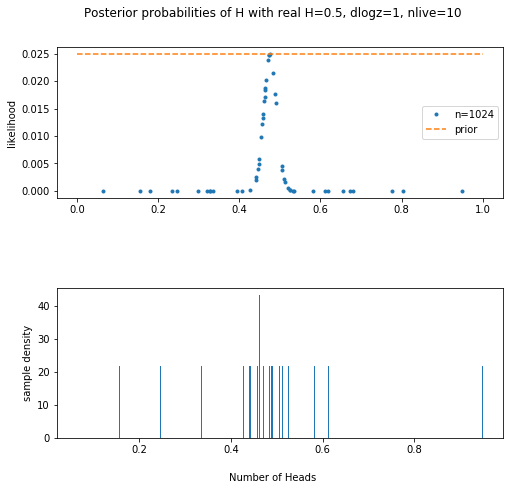
\includegraphics[width=.9\linewidth]{./obipy-resources/692Tys.png}

\begin{minted}[frame=lines,fontsize=\scriptsize]{python}
print(maxL)
\end{minted}

\begin{verbatim}
0.47604769589713536
\end{verbatim}

Now let's try doing this for some higher value of nlive:

\begin{minted}[frame=lines,fontsize=\scriptsize]{python}
maxL = get_and_plot_H(.5, uniform_prior, 1, 25)
\end{minted}

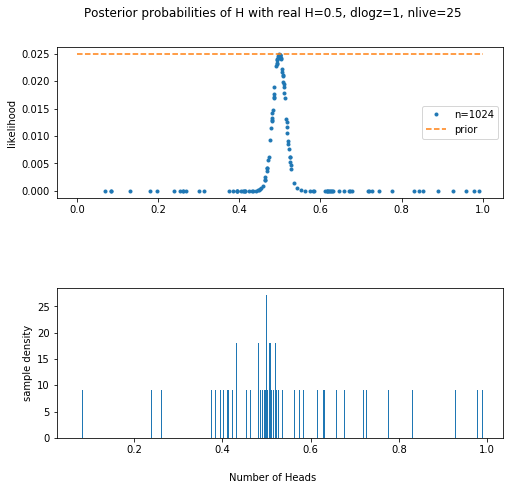
\includegraphics[width=.9\linewidth]{./obipy-resources/692SGC.png}

\begin{minted}[frame=lines,fontsize=\scriptsize]{python}
print(maxL)
\end{minted}

\begin{verbatim}
0.497895669562484
\end{verbatim}

\begin{minted}[frame=lines,fontsize=\scriptsize]{python}
maxL = get_and_plot_H(.5, uniform_prior, 1, 50)
\end{minted}

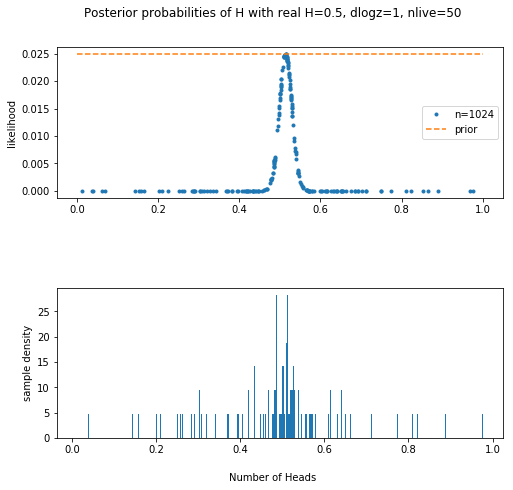
\includegraphics[width=.9\linewidth]{./obipy-resources/692fQI.png}

\begin{minted}[frame=lines,fontsize=\scriptsize]{python}
maxL
\end{minted}

\begin{verbatim}
0.5139972296763047
\end{verbatim}

\begin{minted}[frame=lines,fontsize=\scriptsize]{python}
maxL = get_and_plot_H(.5, uniform_prior, 1, 500)
\end{minted}

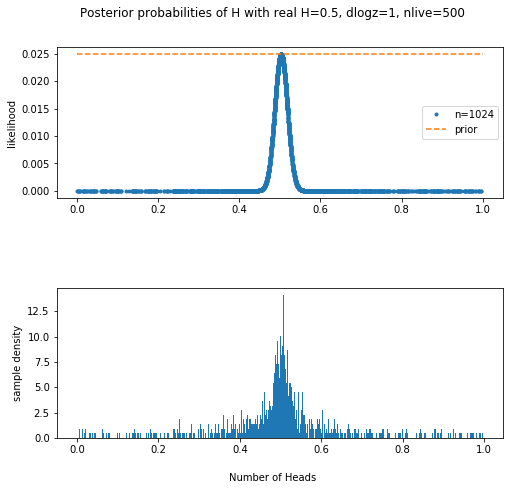
\includegraphics[width=.9\linewidth]{./obipy-resources/692saO.png}

\begin{minted}[frame=lines,fontsize=\scriptsize]{python}
maxL
\end{minted}

\begin{verbatim}
0.5029426514479755
\end{verbatim}

Now we'll look at a smaller value of dlogz:

\begin{minted}[frame=lines,fontsize=\scriptsize]{python}
maxL = get_and_plot_H(.5, uniform_prior, .1, 500)
\end{minted}

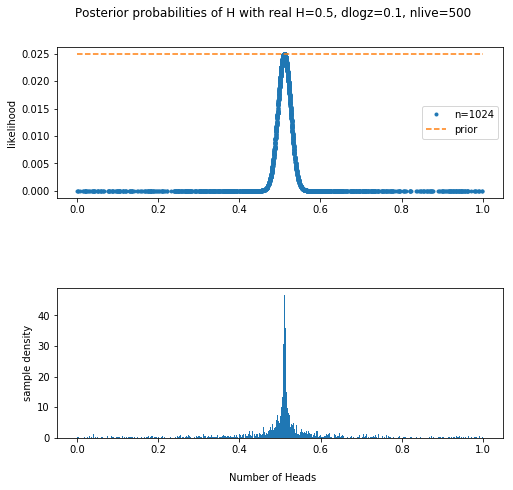
\includegraphics[width=.9\linewidth]{./obipy-resources/692gDn.png}

\begin{minted}[frame=lines,fontsize=\scriptsize]{python}
maxL
\end{minted}

\begin{verbatim}
0.5107393662844353
\end{verbatim}

Here we're getting pretty close now to the actual value of H.
Now we can start working non-uniform priors:
\end{itemize}

\subsubsection*{Gaussian Priors}
\label{sec-1-3-2}

\begin{minted}[frame=lines,fontsize=\scriptsize]{python}
def gaussian(x, mu=0, sigma=1, C=1):
    return C * np.exp((-(x - mu) ** 2) / (2 * sigma ** 2))
\end{minted}


\begin{minted}[frame=lines,fontsize=\scriptsize]{python}
get_and_plot_H(.5, gaussian, .1, 500, mu=.5, sigma=.25)
\end{minted}

\begin{verbatim}
0.5039108982035918
\end{verbatim}
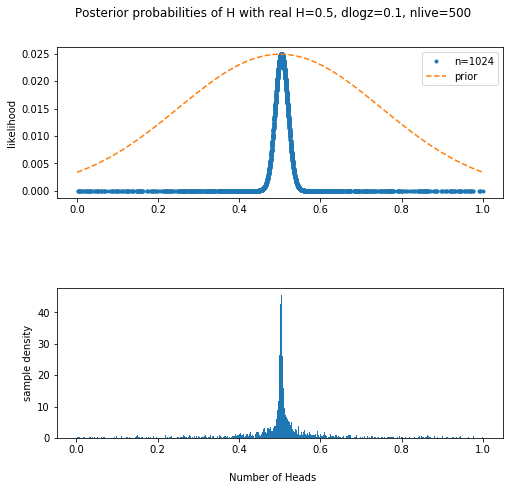
\includegraphics[width=.9\linewidth]{./obipy-resources/6926Xz.png}

\begin{minted}[frame=lines,fontsize=\scriptsize]{python}
get_and_plot_H(.7, gaussian, .1, 500, mu=.5, sigma=.25)
\end{minted}

\begin{verbatim}
0.704096061543153
\end{verbatim}
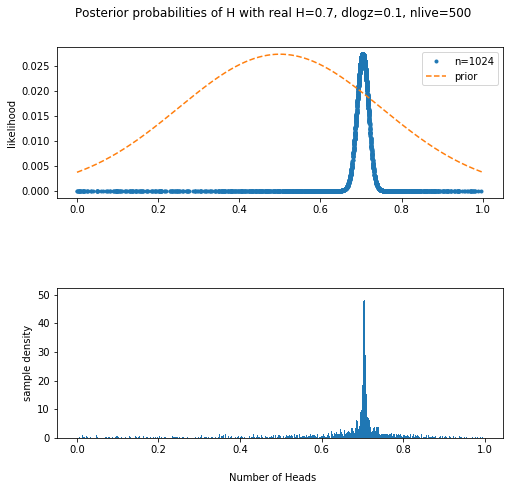
\includegraphics[width=.9\linewidth]{./obipy-resources/692shC.png}

\begin{minted}[frame=lines,fontsize=\scriptsize]{python}
get_and_plot_H(.7, gaussian, .1, 500, mu=.3, sigma=.1)
\end{minted}

\begin{verbatim}
0.6943432292672936
\end{verbatim}
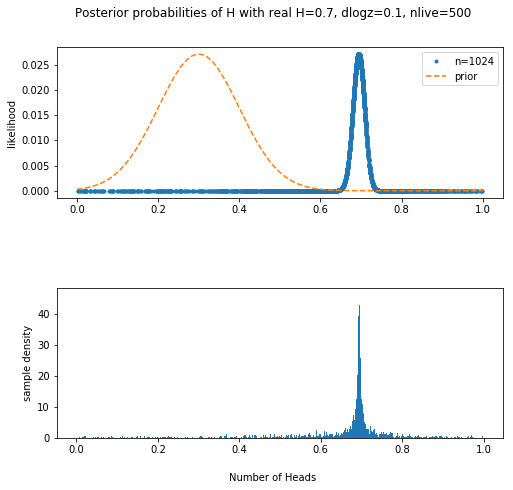
\includegraphics[width=.9\linewidth]{./obipy-resources/6925rI.png}

\section*{Problem 2}
\label{sec-2}
Now we'll look at the lighthouse problem again:

\subsection*{Methods from Previous Set}
\label{sec-2-1}

\begin{minted}[frame=lines,fontsize=\scriptsize]{python}
sults raw drawer
def rand_angle(size=None):
    return np.random.random(size=size) * np.pi - np.pi / 2

def get_theta(d, alpha, beta):
    return np.arctan((d - alpha) / beta)

def get_prob(d, alpha, beta):
    # assume d has been rounded to two places i.e. 1.22
    # range is then 1.215 to 1.225
    high_bound = get_theta(d + .005, alpha, beta)
    low_bound = get_theta(d - .005, alpha, beta)
    diff = np.abs(high_bound - low_bound)
    # this is basically our unnormalized probability
    return diff
    
def get_rand_locs(nlocs, alpha, beta):
    angles = rand_angle(size=nlocs)
    # have that alpha - loc = beta * tan(theta)
    diff = beta * np.tan(angles)
    loc = alpha - diff
    return loc

def get_log_likelihood(rounded_data, alpha, beta):
    log_like = np.sum(np.log(np.array(
        [get_prob(d, alpha, beta) for d in rounded_data])))
    return log_like
\end{minted}

\subsection*{MCMC Runs}
\label{sec-2-2}

\begin{minted}[frame=lines,fontsize=\scriptsize]{python}
def plot_lighthouse_corner(results):
    fig = plt.subplots(2, 2, figsize=(10, 6))
    dyplot.cornerplot(results, fig=fig)
    fig[1][1, 0].set_ylabel(r'$\beta$')
    fig[1][1, 0].set_xlabel(r'$\alpha$')
    fig[1][1, 1].set_xlabel(r'$\beta$')
    plt.tight_layout()
    plt.show()

def plot_lighthouse_scatter(results):
    fig = plt.subplots(1, 1, figsize=(8, 5))
    dyplot.cornerpoints(results, fig=fig)
    fig[1].set_ylabel(r'$\beta$')
    fig[1].set_xlabel(r'$\alpha$')
    plt.tight_layout()
    plt.xlim(-10, 10)
    plt.ylim(0, 10)
    plt.show()

def plot_traceplot(results):
    fig = plt.subplots(2, 2, figsize=(10, 6))
    dyplot.traceplot(results, fig=fig)
    fig[1][1, 1].set_xlabel(r'$\beta$')
    fig[1][0, 1].set_xlabel(r'$\alpha$')
    fig[1][1, 0].set_ylabel(r'$\beta$')
    fig[1][0, 0].set_ylabel(r'$\alpha$')
    plt.tight_layout()
    plt.show()

def plot_runplot(results):
    dyplot.runplot(results)
    plt.show()
\end{minted}


We'll stick with an nlive value of 500 and a dlogz value of .01:

\begin{minted}[frame=lines,fontsize=\scriptsize]{python}
def get_grid_posts(n, alpha, beta, dlogz_val=.1, interloper=False, d=1):
    locs = np.round(get_rand_locs(n, alpha, beta), 2)
    if (interloper):
        interloper_locs= np.round(get_rand_locs(n, alpha + d, beta - d), 2)
        locs = np.append(locs, interloper_locs)
    
    def lighthouse_logl(params):
        return get_log_likelihood(locs, params[0], params[1])
    
    # here we'll really just keep it uniform from (-100, 100)
    def ptform(u):
        return [2000 * u[0] - 1000, 1000 * u[1]]

    ndim = 2
    sampler = dynesty.NestedSampler(lighthouse_logl, ptform, ndim,
                                           bound='single', nlive=500) 

    sampler.run_nested(dlogz=dlogz_val, print_progress=False)
    return sampler.results
\end{minted}


First we'll just look at the original lighthouse problem:

\begin{minted}[frame=lines,fontsize=\scriptsize]{python}
results = get_grid_posts(500, 0, 5)
\end{minted}


\begin{minted}[frame=lines,fontsize=\scriptsize]{python}
plot_lighthouse_corner(results)
plt.show()
\end{minted}

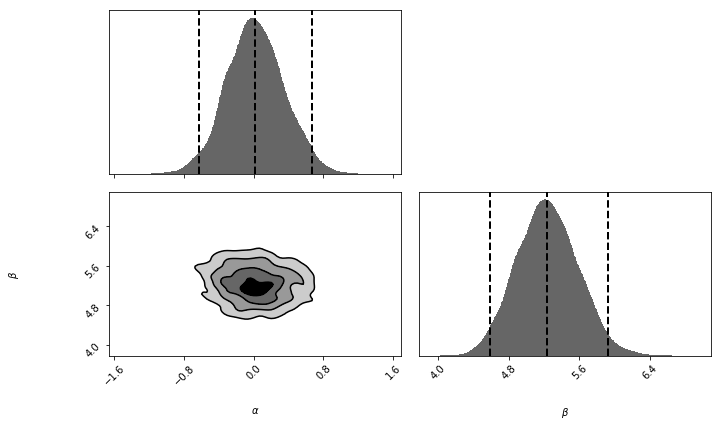
\includegraphics[width=.9\linewidth]{./obipy-resources/692Ghy.png}

\begin{minted}[frame=lines,fontsize=\scriptsize]{python}
plot_lighthouse_scatter(results)
\end{minted}

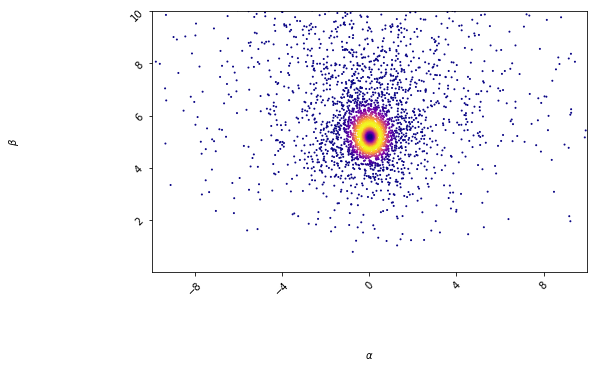
\includegraphics[width=.9\linewidth]{./obipy-resources/6924qB.png}

\begin{minted}[frame=lines,fontsize=\scriptsize]{python}
plot_traceplot(results)
\end{minted}

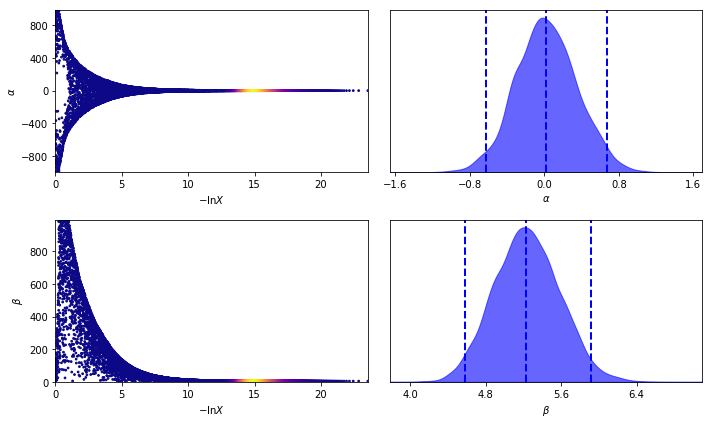
\includegraphics[width=.9\linewidth]{./obipy-resources/692F1H.png}

\begin{minted}[frame=lines,fontsize=\scriptsize]{python}
plot_runplot(results)
\end{minted}

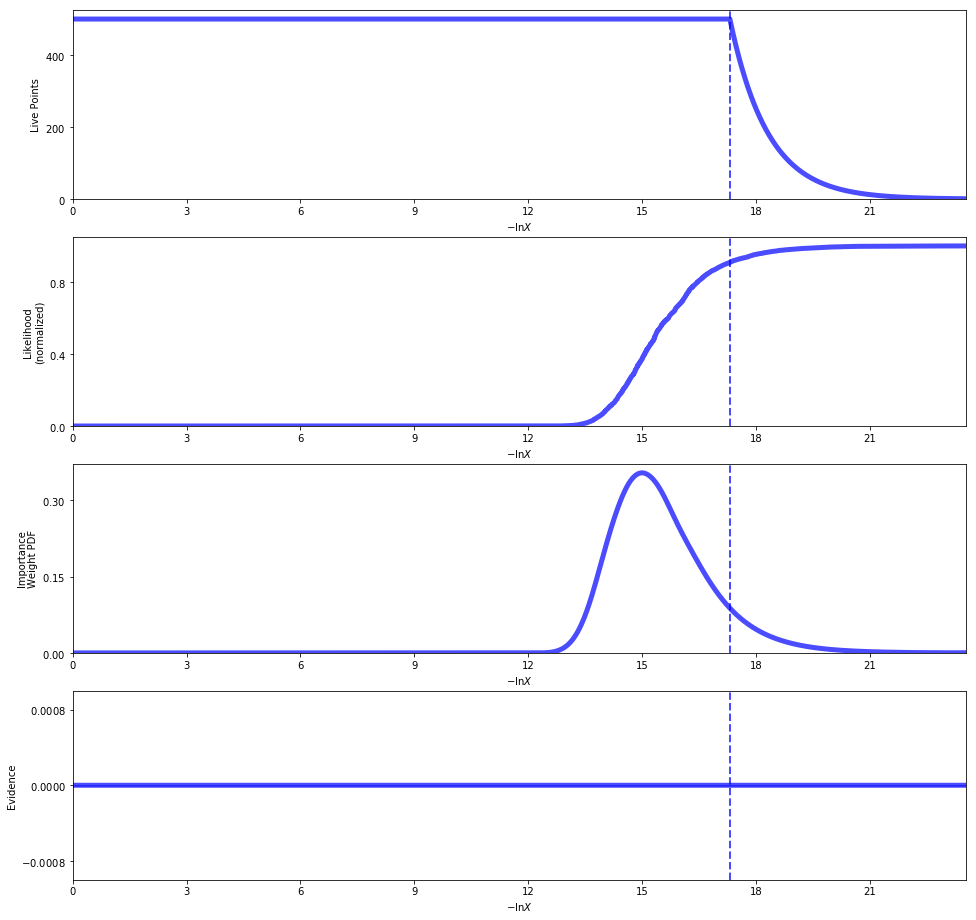
\includegraphics[width=.9\linewidth]{./obipy-resources/692S_N.png}

\begin{minted}[frame=lines,fontsize=\scriptsize]{python}
results.samples[-1]
\end{minted}

\begin{verbatim}
array([0.03130404, 5.18680251])
\end{verbatim}

Here we see that we get pretty close to the 'correct' values of (0, 5).

Now let's try looking at the interloper case located at (1, 4):

\begin{minted}[frame=lines,fontsize=\scriptsize]{python}
interloper_results = get_grid_posts(500, 0, 5, interloper=True)
\end{minted}


\begin{minted}[frame=lines,fontsize=\scriptsize]{python}
plot_lighthouse_corner(interloper_results)
\end{minted}

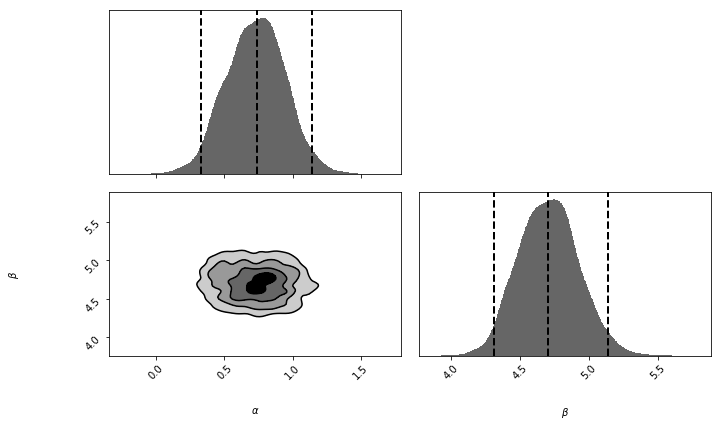
\includegraphics[width=.9\linewidth]{./obipy-resources/692fJU.png}

\begin{minted}[frame=lines,fontsize=\scriptsize]{python}
plot_runplot(interloper_results)
\end{minted}

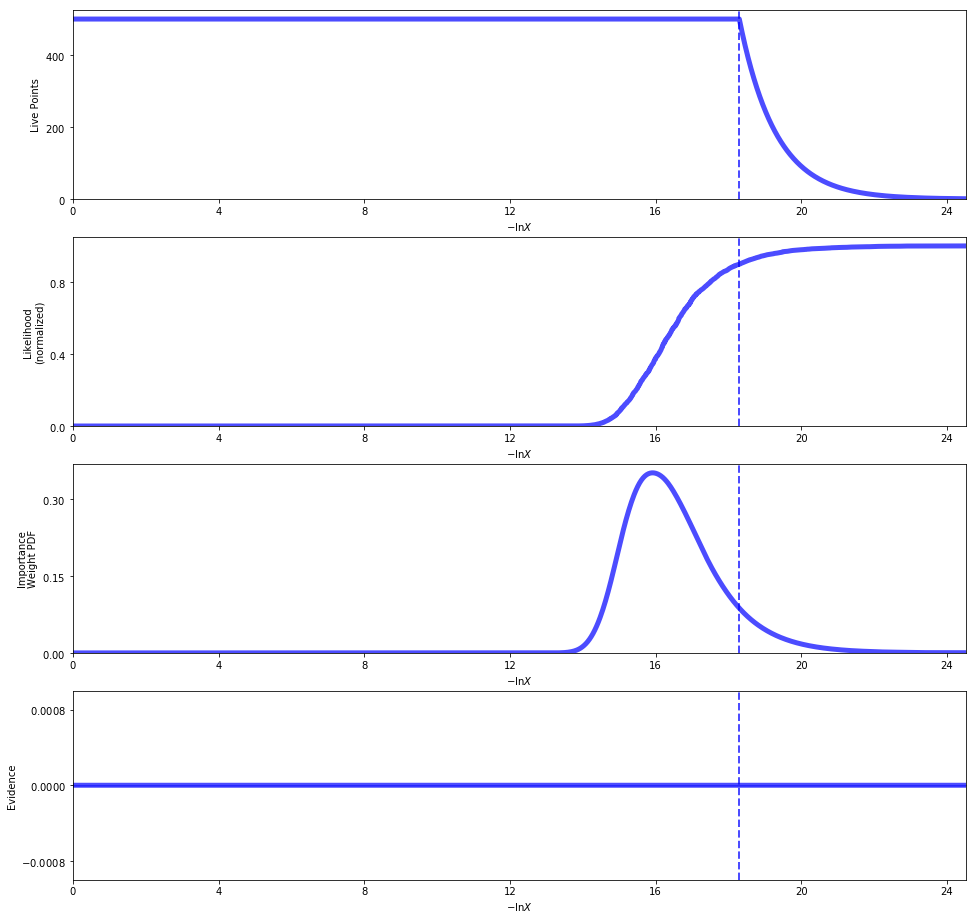
\includegraphics[width=.9\linewidth]{./obipy-resources/692G2O.png}

Here we see that it's pretty hard to actually splot this interloper
here. Instead the $\alpha$ and $\beta$ values are just in-between the two values of
the original lighthouse and interloper.

Maybe a larger discrepancy between original and interloper would be better,
this time with the original located at (0, 7) and the interloper located at (5,
2):

\begin{minted}[frame=lines,fontsize=\scriptsize]{python}
larger_interloper_results = get_grid_posts(500, 0, 7, interloper=True, d=5)
\end{minted}


\begin{minted}[frame=lines,fontsize=\scriptsize]{python}
plot_lighthouse_corner(larger_interloper_results)
\end{minted}

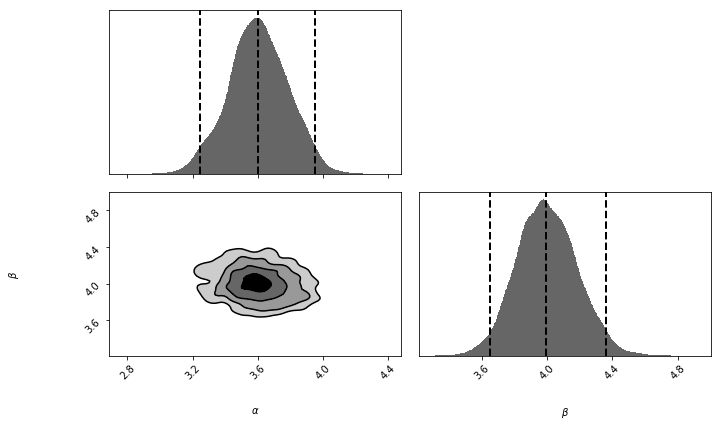
\includegraphics[width=.9\linewidth]{./obipy-resources/692sTa.png}

\begin{minted}[frame=lines,fontsize=\scriptsize]{python}
plot_runplot(larger_interloper_results)
\end{minted}

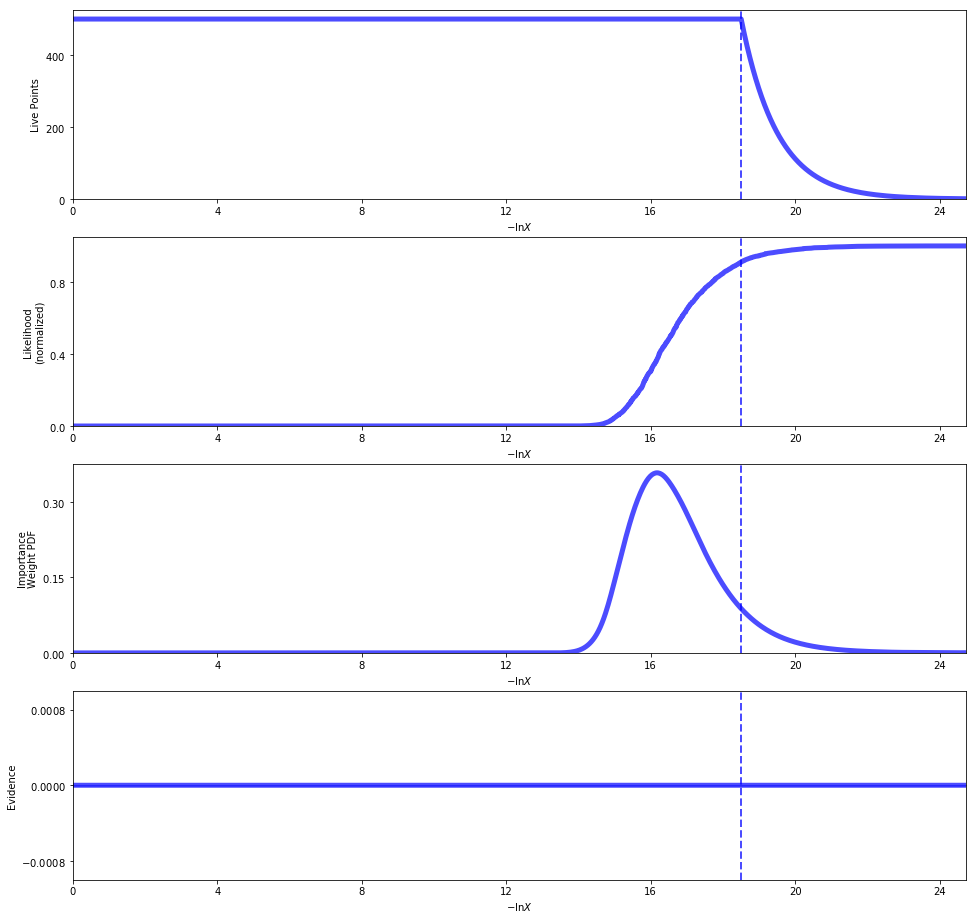
\includegraphics[width=.9\linewidth]{./obipy-resources/692TAV.png}

Here we also are unable to find this interloper. Even weirder is the fact that
our $\alpha$ and $\beta$ values are not even near the means of the values of the
two lighthouses: $\alpha$ is above while $\beta$ is below.
% Emacs 25.2.1 (Org mode 8.2.10)
\end{document}
